\documentclass[tikz,border=2pt]{standalone}
\usepackage{unicode-math}
\setmainfont[
  Path=publication/fonts/,
  UprightFont=source-serif-4-latin-400-normal.ttf,
  ItalicFont=source-serif-4-latin-400-italic.ttf,
  BoldFont=source-serif-4-latin-600-normal.ttf,
  BoldItalicFont=source-serif-4-latin-600-italic.ttf
]{Source Serif 4}
\setmathfont[Path=/System/Library/Fonts/Supplemental/]{STIXTwoMath.otf}
\usepackage{tikz}
\usetikzlibrary{arrows.meta,backgrounds,calc,decorations.pathreplacing,fit,matrix,positioning}
\definecolor{BookInk}{HTML}{18232D}
\definecolor{BookBlue}{HTML}{315F78}
\definecolor{BookRed}{HTML}{98452F}
\definecolor{BookGreen}{HTML}{3F6659}
\definecolor{BookMuted}{HTML}{66727A}
\definecolor{BookRule}{HTML}{AEB7BC}
\tikzset{
  book/node/.style={
    draw=BookInk, line width=.55pt, fill=white,
    minimum height=9mm, inner xsep=5pt, inner ysep=4pt,
    font=\footnotesize, align=center
  },
  book/primary/.style={book/node, draw=BookBlue},
  book/decision/.style={book/node, draw=BookRed},
  book/verified/.style={book/node, draw=BookGreen},
  book/arrow/.style={
    -{Stealth[length=2mm,width=1.35mm]}, line width=.55pt, draw=BookInk
  },
  book/quietarrow/.style={
    -{Stealth[length=2mm,width=1.35mm]}, line width=.45pt, draw=BookRule
  },
  book/feedback/.style={
    -{Stealth[length=2mm,width=1.35mm]}, line width=.5pt,
    draw=BookRed, dashed
  },
  book/note/.style={font=\scriptsize, text=BookMuted, align=center}
}

\begin{document}
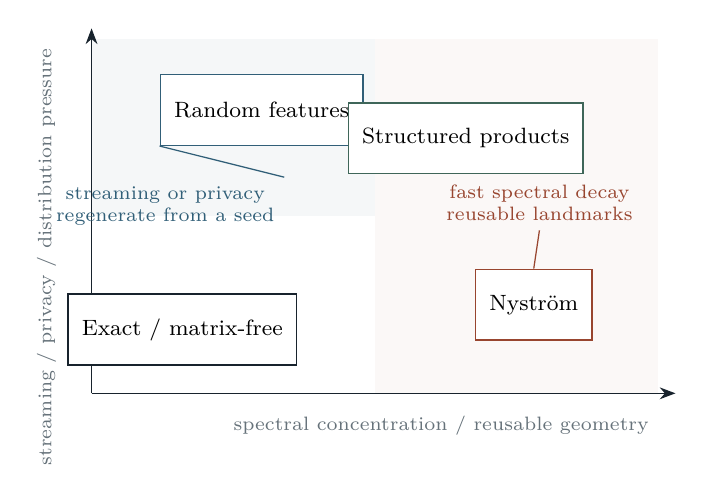
\begin{tikzpicture}[x=7.2cm,y=4.5cm]
  \fill[BookBlue!5] (0,.5) rectangle (1,1);
  \fill[BookRed!4] (.5,0) rectangle (1,1);
  \draw[BookInk,line width=.5pt,-{Stealth[length=2mm]}] (0,0)--(1.03,0);
  \draw[BookInk,line width=.5pt,-{Stealth[length=2mm]}] (0,0)--(0,1.03);
  \node[book/note,anchor=north east] at (1,-.035)
    {spectral concentration / reusable geometry};
  \node[book/note,rotate=90,anchor=south east] at (-.045,1)
    {streaming / privacy / distribution pressure};
  \node[book/node] at (.16,.18) {Exact / matrix-free};
  \node[book/decision] (nys) at (.78,.25) {Nyström};
  \node[book/primary] (rff) at (.30,.80) {Random features};
  \node[book/verified] at (.66,.72) {Structured products};
  \node[book/note,text=BookRed,anchor=south] (nysnote) at (.79,.46)
    {fast spectral decay\\reusable landmarks};
  \draw[BookRed,line width=.45pt] (nysnote.south)--(nys.north);
  \node[book/note,text=BookBlue,anchor=north] (rffnote) at (.13,.61)
    {streaming or privacy\\regenerate from a seed};
  \draw[BookBlue,line width=.45pt] (rffnote.north east)--(rff.south west);
\end{tikzpicture}
\end{document}
